\documentclass[a4paper,UTF8]{article}
\usepackage{ctex}
\usepackage[margin=1.25in]{geometry}
\usepackage{color}
\usepackage{graphicx}
\usepackage{amssymb}
\usepackage{amsmath}
\usepackage{amsthm}
\usepackage{enumerate}
\usepackage{bm}
\usepackage{hyperref}
\usepackage{pgfplots}
\usepackage{epsfig}
\usepackage{color}
\usepackage{tcolorbox}
\usepackage{mdframed}
\usepackage{lipsum}
\newmdtheoremenv{thm-box}{myThm}
\newmdtheoremenv{prop-box}{Proposition}
\newmdtheoremenv{def-box}{定义}

\setlength{\evensidemargin}{.25in}
\setlength{\textwidth}{6in}
\setlength{\topmargin}{-0.5in}
\setlength{\topmargin}{-0.5in}
% \setlength{\textheight}{9.5in}
%%%%%%%%%%%%%%%%%%此处用于设置页眉页脚%%%%%%%%%%%%%%%%%%
\usepackage{fancyhdr}                                
\usepackage{lastpage}                                   
\usepackage{layout}                                     
\newtheorem*{solution}{Solution}

\footskip = 10pt 
\pagestyle{fancy}                    % 设置页眉                 
\lhead{2020年秋季}                    
\chead{高级机器学习}                                                
% \rhead{第\thepage/\pageref{LastPage}页} 
\rhead{作业一}                                                                                               
\cfoot{\thepage}                                                
% \renewcommand{\headrulewidth}{1pt}  			%页眉线宽,设为0可以去页眉线
\setlength{\skip\footins}{0.5cm}    			%脚注与正文的距离           
% \renewcommand{\footrulewidth}{0pt}  			%页脚线宽,设为0可以去页脚线

\makeatletter 									%设置双线页眉                                        
\def\headrule{{\if@fancyplain\let\headrulewidth\plainheadrulewidth\fi%
\hrule\@height 1.0pt \@width\headwidth\vskip1pt	%上面线为1pt粗  
\hrule\@height 0.5pt\@width\headwidth  			%下面0.5pt粗            
\vskip-2\headrulewidth\vskip-1pt}      			%两条线的距离1pt        
 \vspace{6mm}}     								%双线与下面正文之间的垂直间距              
\makeatother  

%%%%%%%%%%%%%%%%%%%%%%%%%%%%%%%%%%%%%%%%%%%%%%
\numberwithin{equation}{section}
%\usepackage[thmmarks, amsmath, thref]{ntheorem}
\newtheorem{myThm}{myThm}
\newtheorem*{myDef}{Definition}
\newtheorem*{mySol}{Solution}
\newtheorem*{myProof}{Proof}
\newtheorem*{myRemark}{备注}
% \renewcommand{\tilde}{\widetilde}
% \renewcommand{\hat}{\widehat}
\newcommand{\indep}{\rotatebox[origin=c]{90}{$\models$}}
\newcommand*\diff{\mathop{}\!\mathrm{d}}

\usepackage{multirow}

%--

%--
\begin{document}
\title{高级机器学习\\
作业一}
\author{丁豪\, 181220010} 
\maketitle
%%%%%%%% 注意: 使用XeLatex 编译可能会报错,请使用 pdfLaTex 编译 %%%%%%%

\section*{学术诚信}

本课程非常重视学术诚信规范,助教老师和助教同学将不遗余力地维护作业中的学术诚信规范的建立。希望所有选课学生能够对此予以重视。\footnote{参考尹一通老师\href{http://tcs.nju.edu.cn/wiki/}{高级算法课程}中对学术诚信的说明。}

\begin{tcolorbox}
	\begin{enumerate}
		\item[(1)] 允许同学之间的相互讨论,但是{\color{red}\textbf{署你名字的工作必须由你完成}},不允许直接照搬任何已有的材料,必须独立完成作业的书写过程;
		\item[(2)] 在完成作业过程中,对他人工作(出版物、互联网资料)中文本的直接照搬(包括原文的直接复制粘贴及语句的简单修改等)都将视为剽窃,剽窃者成绩将被取消。{\color{red}\textbf{对于完成作业中有关键作用的公开资料,应予以明显引用}};
		\item[(3)] 如果发现作业之间高度相似将被判定为互相抄袭行为,{\color{red}\textbf{抄袭和被抄袭双方的成绩都将被取消}}。因此请主动防止自己的作业被他人抄袭。
	\end{enumerate}
\end{tcolorbox}

\section*{作业提交注意事项}
\begin{tcolorbox}
	\begin{enumerate}
		\item[(1)] 请在LaTeX模板中{\color{red}\textbf{第一页填写个人的姓名、学号、邮箱信息}};
		\item[(2)] 本次作业需提交该pdf文件、问题3可直接运行的源码(学号\_.py),将以上两个文件压缩成zip文件后上传。zip文件格式为{\color{red}\textbf{学号.zip}},例如170000001.zip;pdf文件格式为{\color{red}\textbf{学号\_姓名.pdf}},例如170000001\_张三.pdf。
		\item[(3)] 未按照要求提交作业,或提交作业格式不正确,将会{\color{red}\textbf{被扣除部分作业分数}};
		\item[(4)] 本次作业提交截止时间为{\color{red}\textbf{11月8日23:59:59}}。除非有特殊情况(如因病缓交),否则截止时间后不接收作业,本次作业记零分。
	\end{enumerate}
\end{tcolorbox}

\newpage
\section{[30pts] VC Dimensions}
本题探讨~VC~维的性质。

\begin{enumerate}[(1)]
	\item \textbf{[10pts]} 请在样本空间~$\mathcal{X} = [0,1]$~上构造一个有限假设空间~$\mathcal{H}$~使得~$\mbox{VC}(\mathcal{H}) = \left \lfloor \log_2(\left| \mathcal{H} \right| ) \right \rfloor $.
	\item \textbf{[10pts]} 定义轴平行四边形概念类~$\mathcal H = \{h_{(a_1, a_2, b_1, b_2)}(x, y): a_1\le a_2 \land b_1\le b_2\}$, 其中
	\[ h_{(a_1, a_2, b_1, b_2)}(x, y) = \begin{cases}
	1&\quad \text{ if } a_1\le x\le a_2 \land b_1\le y \le b_2 \\
	0 & \quad \text{otherwise}
	\end{cases}
	\]
	请证明~$\mathcal H$~的~VC~维为~4.
	\item \textbf{[10 pts]} 请证明最近邻分类器的假设空间的~VC~维可以为无穷大.
\end{enumerate}

\begin{solution}
此处用于写解答(中英文均可)
\begin{enumerate}[(1)]
    \item $\mathcal H = \{h_1,h_2,h_3,h_4\}$,其中
        $$h_1(x)=\begin{cases}
            0& \text{x>=-1}\\
            1& \text{x<-1}
        \end{cases},
        h_2(x)=\begin{cases}
            1& \text{x>=-1}\\
            0& \text{x<-1}
        \end{cases},
        h_3(x)=\begin{cases}
            1& \text{x>=0.5}\\
            0& \text{x<0.5}
        \end{cases},
        h_4(x)=\begin{cases}
            0& \text{x>=0.5}\\
            1& \text{x<0.5}
        \end{cases}$$
        则存在$D=\{x_1=0.2,x_2=0.7\}$,则其可以被$\mathcal H$打散。对任意大小为3的示例集$\{x_3,x_4,x_5\}$,不妨设$x_3<x_4<x_5$,则$\mathcal H$中不存在任何假设
        能实现对分结果$(1,0,1)$。因此$VC(\mathcal H) = 2 =\lfloor log_2(|\mathcal H|) \rfloor$
    \item 存在 $D = \{(0,-1),(-1,0),(0,1),(1,0)\}$,则假设空间中存在$\{h_{(0,0,0,0)},h_{(-1,-1,0,0)},h_{(1,1,0,0)},\\
        h_{(0,0,1,1)},h_{(0,0,-1,-1)},h_{(-1,0,0,1)},h_{(0,1,0,1)},h_{(-1,0,-1,0)},h_{(0,1,-1,0)},h_{(-1,1,0,0)},h_{(0,0,-1,1)},\\
        h_{(-1,0,-1,1)},h_{(-1,1,0,1)},h_{(0,1,-1,1)},h_{(-1,1,-1,0)},h_{(1,1,1,1)}\}$ 可以将$D$对分,因此$VC(\mathcal H) \ge 4.$\\
        与此同时,对任意大小为5的示例集$\{(x_1,y_1),(x_2,y_2),(x_3,y_3),(x_4,y_4),(x_5,y_5)\}$,不妨设$x_1 \le x_2 \le x_3 \le x_4 \le x_5$.
        若$\mathcal H$可以打散$D$,则对任意$(x_i,x_j),(x_x,x_y,x_z)$的组合,存在某$h\in \mathcal H$使得$h(x_i)=h(x_j)=1 \wedge h(x_x)=h(x_y)=h(x_z)=0$,
        即可以用边平行于X、Y轴的矩形将坐标平面上的5个点每两个与其余分隔开。由图论知识可以证明,这是不可能的,因而不存在这样的D。所以$\mathcal H$的VC纬为4.
    \item 对任意m,设某示例集$D=\{x_1,x_2 \dots x_m\}$,考虑$\mathcal H$中以$\{(x_1,y_1),(x_2,y_2) \dots (x_m,y_m)\}$为邻居点产生的分类器$\{h\}$,$h|_D=\{y_1,y_2\dots y_m\}$,则共有$2^m$种可能结果(对$y_i$二进制赋值得到),
        即$\mathcal H$可以将$D$打散,所以$VC(\mathcal H) \ge m$。由于对任意m都成立,因此最近邻分类器的假设空间VC纬可以为正无穷。
\end{enumerate}
\end{solution}

\section{\textbf{[40pts]} Understanding the Parameters in LVW from A Probabilistic Perspective}
课程中,我们介绍了一种包裹式特征选择算法Las Vegas Wrapper(简称LVW),该算法的流程如教材中图11.1所示。首先请各位回顾一下LVW算法,接下来我们将对一种特殊情况下的LVW做一些分析,过程中复习一些简单的概率知识,并从更理性的角度理解LVW中的参数。

现在,我们获得了一个数据集$D$,该数据集中一共包含$N$个特征,设特征集合为$A=\{f_1,f_2,\cdots,f_N\}$。我们知道,对于某个具体任务,特征的质量参差不齐,高质量的特征会带来高质量的性能,低质量的特征会带来低质量的性能。我们设第$i$个特征的质量为$2^{i-1}$,即$N$个特征的质量分别为$1,2,4,\cdots,2^{N-1}$。我们规定:给定一个特征子集$A^\prime$,学习器在$A^\prime$上的性能恰好等于$A^\prime$中包含的所有特征的质量之和。设特征子集$A^\prime$中特征的质量之和记作$Q(A^\prime)$。

\begin{enumerate}[(1)]
\item \textbf{[5pts]} 现执行一次图11.1中第$6$行的语句,产生一个特征子集$A^\prime$,试求数学期望$\mathbb{E}[Q(A^\prime)]$。

\item \textbf{[10pts]} 现在,LVW算法已经执行了一段时间了,当前得到的最优特征子集为$B$,我们记$R=Q(B)$。设函数$better(n,r)$表示从前$n$个特征中随机产生一个特征子集且该特征子集的质量大于$r$的概率。试求$better(N,R)$。这里我们允许以递归式和递归边界来表达$better(N,R)$。
    
\item \textbf{[10pts]} 从现在开始,我们设$better(n,r)$是一个已知函数。在LVW算法中,当连续$T$个随机生成的子集不比当前的最优子集更好时,算法结束。我们仍然设当前得到的最优特征子集为$B$,$B$的质量为$R=Q(B)$。在本小问中,我们还设$T$是一个已知参数。设布尔型随机变量$e$,$p(e=1|T)$表示经过恰好$T$次循环后LVW算法结束的概率,$p(e=0|T)$表示经过恰好$T$次循环后LVW算法没有结束的概率。试求分布$p(e|T)$。

\item \textbf{[5pts]} 由第(3)小问可见,参数$T$越大,LVW算法结束就越([回答“容易”或“困难”]);当前最优子集质量越高,LVW算法结束就越([回答“容易”或“困难”])。

\item \textbf{[10pts]} 现在,我们引入Bayes观点,认为参数$T$是服从某个先验分布$p(T)$的随机变量,且是未知的。我们仍然设当前得到的最优子集为$B$,$B$的质量为$R=Q(B)$。现在,LVW算法继续执行,在恰好执行了$T$个循环后成功退出了。如果我们设$T$的先验分布为整数区间$[1, 10]$上的均匀分布,请对$T$做最大后验估计。这与最大似然估计的结果相同吗?为什么?

\item \textbf{[Bonus 5pts]} 现在,设随机变量$T$只能在$\{1,2,3\}$中取值,且小明设置了一个先验$p(T)$。小红观察到,当前得到的最优子集为$B$,$B$的质量为$R=Q(B)$,且LVW在执行恰好$T$个循环后成功退出了,于是小红试图对$T$做最大后验估计。小红发现,$T$的后验概率在$\{1,2,3\}$上是均匀的,那么小明设置的先验$p(T)$有可能为:(填写一种可能的答案即可)
\begin{table}
	\centering
    \begin{tabular}{|l|l|l|}
        \hline
        $p(T=1)$ & $p(T=2)$ & $p(T=3)$ \\ \hline
        ~      & ~      & ~      \\
        \hline
    \end{tabular}
\end{table}
\end{enumerate}

\begin{solution}
此处用于写解答(中英文均可)
\begin{enumerate}[(1)]
    \item 每一个特征以$\frac{2^{N-1}}{2^N-1}$的概率被选取(分母减去1是去掉了空集的情况),则\\
        $E[Q(A^\prime)]=\sum\limits_{i=1}^N\frac{2^{N-1}}{2^N-1}\cdot 2^{i-1}=\frac{2^{N-1}}{2^N-1}\cdot \frac{1-2^N}{1-2}=2^{N-1}$
    \item $better(N,R)$ 通过以下式子中$n=N,r=R=Q(B)$解出。
        $$better(n,r) = \begin{cases}
        \frac {2^{N-1}-1}{2^N-1} \cdot better(n-1,r)+\frac{2^{N-1}}{2^N-1}\cdot better(n-1,r-2^{n-1}) & ,n \ge 2\\
        \frac{2^{N-1}}{2^N-1} & ,n=1 \wedge r < 1 \\
        0 &,n=1 \wedge r \ge 1
    \end{cases}$$
    通过将题目设定的$R_i=2^{i-1}$代入,可以将递归式化为一般表达式$better(N,R)=\frac{2^N-1-R}{2^N-1}$
    \item $p(e=1|T)=[1-better(N,R)]^T$\\
        $ p(e=0)=1-[1-better(N,R)]^T$
    \item 困难,容易
    \item 为了以示区别,设恰好执行了$T = T_0$个循环后成功退出。\\
        最大后验估计:$\hat T_{MAP}(T_0) = \mathop{\arg\max}\limits_{T\in[1,10],T \in \mathbb N} P(T|T_0)=\mathop{\arg\max}\limits_{T\in[1,10],T \in \mathbb N} P(T_0|T)P(T)$\\
        由于是均匀先验,$P(T)$为定值,因此$\hat T_{MAP}(T_0) = \mathop{\arg\max}\limits_{T\in[1,10],T \in \mathbb N} [1-better(N,R)]^T$\\
        极大似然估计:$\hat T_{MLE}(T_0) = \mathop{\arg\max}\limits_{T \in \mathbb N^+} P(T_0|T)= \mathop{\arg\max}\limits_{T \in \mathbb N^+} [1-better(N,R)]^T$\\
        如果认为最大似然估计的T也需要符合$[1,10]$约束,则表达式完全相同,故结果相同。若不然,则二者不同,因为最大后验具有$T\in[1,10] \wedge T\in\mathbb N$限制,因此不可能求出超过10的T。而极大似然则只有$T \in \mathbb N^+$限制,可以求出超过10的T。
    \item 由极大后验估计公式:\\
        $[1-better(N,R)]P(T=1) = [1-better(N,R)]^2P(T=2) $\\
        $= [1-better(N,R)]^3P(T=3)$\\
        $\therefore P(T=1)=[1-better(N,R)]P(T=2)= [1-better(N,R)]^2P(T=3)$\\
        $\therefore P(T=1)=\frac{R}{2^N-1}P(T=2)=\frac{R^2}{(2^N-1)^2}P(T=3)$且$P(T=1)+P(T=2)+P(T=3)=1$\\
        因此一种可能的先验概率为$P(T=1)=\frac{\frac{R^2}{(2^N-1)^2}}{\frac{R^2}{(2^N-1)^2}+\frac{R}{2^N-1}+1},P(T=2)=\frac{\frac{R}{2^N-1}+1}{\frac{R^2}{(2^N-1)^2}+\frac{R}{2^N-1}+1},P(T=3)=\frac{1}{\frac{R^2}{(2^N-1)^2}+\frac{R}{2^N-1}+1}$
\end{enumerate}
\end{solution}

\section{\textbf{[30pts]} Semi-supervised SVM in practice}
参照教材中图13.4所示的TSVM算法,在所提供的半监督数据集上进行训练,报告模型在未标记数据集以及测试集上的性能。

本次实验的数据集为一个二分类的数据集,已提前划分为训练数据和测试数据,其中训练数据划分为有标记数据和无标记数据。数据的特征维度为30,每一维均为数值类型。数据文件的具体描述如下:
\begin{itemize}
    \item \texttt{label\_X.csv,label\_y.csv}分别是有标记数据的特征及其标签。
    \item \texttt{unlabel\_X.csv,unlabel\_y.csv}分别是无标记数据的特征及其标签。
    \item \texttt{test\_X.csv,test\_y.csv}分别是测试数据的特征及其标签。
\end{itemize}

注意,训练阶段只可以使用\texttt{label\_X.csv,label\_y.csv,unlabel\_X.csv}中的数据,其他的数据只可以在测试阶段使用。
\begin{enumerate}[(1)]
    \item  本次实验要求使用Python3编写,代码统一集中在\texttt{tsvm\_main.py}中,通过运行该文件就可以完成训练和测试,并输出测试结果。
    \item 本次实验需要完成以下功能:
    \begin{itemize}
        \item \textbf{[10pts]} 参照教材中图13.4,使用代码实现TSVM算法。要求:
        \begin{enumerate}[1.]
            \item 不允许直接调用相关软件包中的半监督学习方法。
            \item 可以直接调用相关软件包的SVM算法。
            \item 可以使用诸如\texttt{cvxpy}等软件包求解QP问题。
        \end{enumerate}
        \item \textbf{[10pts]} 使用训练好的模型在无标记数据和测试数据上进行预测,报告模型在这两批数据上的准确率和ROC曲线以及AUC值。
        \item \textbf{[10pts]} 尝试使用各种方法提升模型在测试集上的性能,例如数据预处理,超参数调节等。报告你所采取的措施,以及其所带来的提升。
    \end{itemize}
\end{enumerate}
\begin{solution}
此处用于写解答(中英文均可)
\begin{enumerate}
    \item 如181220010\_.py所示,完成了本部分内容。使用了sklearn的svm.SAC包进行软间隔支持向量机求解。同时使用skleran.matrix中的accuracy\_score,roc\_curve,auc函数用于计算评价指标。
    \item 此版本,设置$C_l,C_u$初始值为$1,0.000001$。得到结果为,\\
    在unlabel数据集上$acc=0.9385964912280702, auc=0.9744516129032258$\\
    在test数据集上$acc=0.9557522123893806, auc=0.9838603425559947$\\
    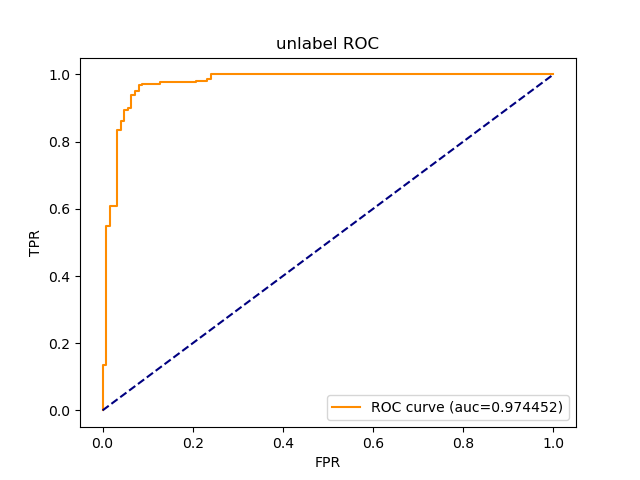
\includegraphics[scale=0.8]{figures/Figure_1.png}\\
    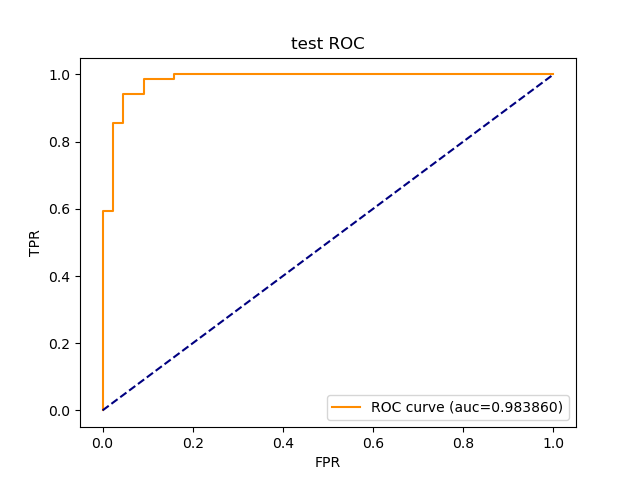
\includegraphics[scale=0.8]{figures/Figure_2.png}
    \item 逐步改进过程如下
    \begin{itemize}
        \item 设置不同的$C_l,C_u$初始值,调整得到最优情况为$1,0.000001$,结果在上一小问已经呈现。
        \item 对数据特征进行标准化,即均值归0,标准差归1。\\
        得到unlabel上$acc=0.9649122807017544,auc=0.9902672811059908$\\
        test上$acc=0.9646017699115044,auc=0.9976943346508564$
    \end{itemize}
\end{enumerate}
\end{solution}
\end{document}